% ============================================================================
% 2000 年春季高考（京、皖）文科 第 23 题：抛物线 y² = 4px 与点 A、B、M
% ----------------------------------------------------------------------------
% 来源：.work/phase4-b20/source/2000春季京皖文.pdf
%       SHA-256 b9552b8354735296f6ea1ed051085e094e4af0c14ff97ada2dbd4e579b14287f
%       第 2 页，内容流对象 2
% 重绘方式：qpdf --qdf 取内容流 → 解析 m/l/c/re/S/f、w、d → 本地坐标
%          本地坐标 = 页面坐标 − (701.132, 687.581)，原点取坐标原点 O；
%          1 单位 = 1 TeX pt；页面为 A3（1190.55 × 841.89 pt）。
% 元素计数：实线路径 8（x 轴、y 轴、抛物线上支、下支、OA、OB、AB、OM），填充箭头 2，虚线 0，标签 6（O, A, B, M, x, y）
% 线宽：轴与辅助线 0.40 pt；抛物线两支 0.80 pt（内容流 w=0.79701）；箭头填充三角形长 3.99 pt、半宽 1.49 pt
% 坐标基准与源位的偏差：端点四舍五入到 0.001 pt；抛物线两支按 24 段三次 Bézier 采样的折线重绘，经 0.02 pt 容差简化（每支 32 点），最大偏差 < 0.02 pt。
% 标签：位置 = pdftotext -bbox 文本中心 − 基准；O、A、B、M、y 未动；x 源位 (68.578,−5.591)，下移 1.6 pt。净距均 ≥ 2 pt
% ============================================================================
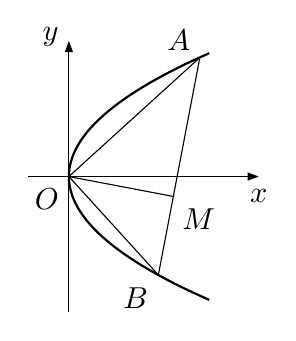
\begin{tikzpicture}[x=1pt, y=1pt,
    every node/.style={inner sep=0pt, font=\fontsize{10.5pt}{12.6pt}\selectfont}]
  % --- 坐标轴（轴身止于箭头底边，箭头为独立填充三角形）
  \draw[line width=0.4pt] (-14.695,0) -- (64.989,0); % x 轴轴身
  \fill (68.576,0) -- (64.591,1.494) -- (64.591,-1.494) -- cycle; % x 箭头
  \draw[line width=0.4pt] (0,-48.983) -- (0,45.396); % y 轴轴身
  \fill (0,48.983) -- (1.494,44.998) -- (-1.494,44.998) -- cycle; % y 箭头
  % --- 抛物线 y^2=4px 上、下两支（内容流 24 段三次 Bézier → 0.02pt 容差 32 点折线）
  \draw[line width=0.8pt]
      (0.000,0.000) -- (0.076,1.712) -- (0.202,2.786) -- (0.408,3.995) -- (0.792,5.572) -- (1.305,7.148) --
      (1.786,8.357) -- (2.337,9.567) -- (3.169,11.143) -- (4.130,12.720) -- (4.955,13.929) -- (5.849,15.138) --
      (7.129,16.715) -- (8.539,18.291) -- (9.708,19.500) -- (10.946,20.710) -- (12.675,22.286) -- (14.532,23.863) --
      (16.045,25.072) -- (17.627,26.281) -- (19.804,27.858) -- (22.110,29.434) -- (23.967,30.644) -- (25.893,31.853) --
      (28.518,33.429) -- (31.272,35.006) -- (33.473,36.215) -- (35.743,37.424) -- (38.816,39.001) -- (42.019,40.577) --
      (44.563,41.787) -- (50.699,44.572);
  \draw[line width=0.8pt]
      (0.000,0.000) -- (0.076,-1.712) -- (0.202,-2.786) -- (0.408,-3.995) -- (0.792,-5.572) -- (1.305,-7.148) --
      (1.786,-8.357) -- (2.337,-9.567) -- (3.169,-11.143) -- (4.130,-12.720) -- (4.955,-13.929) -- (5.849,-15.138) --
      (7.129,-16.715) -- (8.539,-18.291) -- (9.708,-19.500) -- (10.946,-20.710) -- (12.675,-22.286) -- (14.532,-23.863) --
      (16.045,-25.072) -- (17.627,-26.281) -- (19.804,-27.858) -- (22.110,-29.434) -- (23.967,-30.644) -- (25.893,-31.853) --
      (28.518,-33.429) -- (31.272,-35.006) -- (33.473,-36.215) -- (35.743,-37.424) -- (38.816,-39.001) -- (42.019,-40.577) --
      (44.563,-41.787) -- (50.699,-44.572);
  % --- 辅助线：OA、OB、AB、OM
  \draw[line width=0.4pt] (0,0) -- (47.317,43.007);   % OA
  \draw[line width=0.4pt] (0,0) -- (32.329,-35.562);  % OB
  \draw[line width=0.4pt] (32.329,-35.562) -- (47.317,43.007); % AB
  \draw[line width=0.4pt] (0,0) -- (38.108,-7.270);   % OM ⊥ AB
  % --- 标签
  \node at (-7.990,-8.250) {$O$};
  \node at (39.680,49.330) {$A$};
  \node at (24.120,-43.810) {$B$};
  \node at (46.900,-15.520) {$M$};
  \node at (68.580,-7.190) {$x$};
  \node at (-6.650,50.370) {$y$};
\end{tikzpicture}
% ----------------------------------------------------------------------------
% 自验：A=(47.317,43.007) 即页面 (748.449,730.588)、B=(32.329,−35.562) 即 (733.460,652.020)、M=(38.108,−7.270) 即 (739.240,680.311)，均在内容流端点 0.001 pt 内；OA·OB = 0.0（OA⊥OB），OM·AB = 0.0（OM⊥AB，|OM| = 38.795 pt）；两支对 x = 0.025521·y² 的最大残差 0.012 pt（y² = 4px，p ≈ 9.80 pt），两支端点 (50.699,±44.572) 与源 (751.831,732.153)/(751.831,643.009) 吻合。标签：O、A、B、M、y 取源位，x 下移 1.6 pt；净距 O 3.89、A 2.41、B 6.58、M 5.11、x 2.98、y 3.44 pt。探针编译：0 错误、0 警告。
% ============================================================================
